\documentclass[11pt]{article}

\usepackage[T1]{fontenc}
\usepackage[utf8]{inputenc}
\usepackage{lmodern}
\usepackage[margin=1in]{geometry}
\usepackage{setspace}
\usepackage{hyperref}
\usepackage{booktabs}
\usepackage{longtable}
\usepackage{tabularx}
\usepackage{array}
\usepackage{enumitem}
\usepackage{amsmath,amssymb}
\usepackage{tikz}
\usepackage{xcolor}
\usepackage{fancyhdr}
\usetikzlibrary{arrows.meta,positioning,shapes.geometric,shapes.misc,fit,backgrounds}

\hypersetup{
  colorlinks=true,
  linkcolor=blue!50!black,
  urlcolor=blue!50!black,
  pdftitle={Neo Abstract Account Specification},
  pdfauthor={OpenAI Codex for neo-abstract-account repository}
}

\pagestyle{fancy}
\setlength{\headheight}{14pt}
\fancyhf{}
\lhead{Neo Abstract Account Specification}
\rhead{2026-03-09}
\cfoot{\thepage}

\setstretch{1.08}
\setlist[itemize]{leftmargin=1.2em}
\setlist[enumerate]{leftmargin=1.4em}

\newcommand{\code}[1]{\texttt{#1}}
\newcommand{\must}{\textbf{MUST}}
\newcommand{\should}{\textbf{SHOULD}}
\newcommand{\mayword}{\textbf{MAY}}
\newcommand{\aasystem}{Neo Abstract Account}
\newcommand{\AAsystem}{AA}

\title{\textbf{Neo Abstract Account Specification}\\
\large A Formal Implementation-Oriented Specification for Policy-Gated Abstract Accounts on Neo N3}
\author{Repository Specification Draft}
\date{2026-03-09}

\begin{document}
\maketitle
\tableofcontents
\newpage

\section{Abstract}
This document specifies the \aasystem{} reference system implemented in the \code{neo-abstract-account} repository. The system defines a policy-gated abstract account model for Neo N3 in which one shared master contract governs deterministic per-account verify addresses, role- and threshold-based authorization, EVM-compatible meta-transactions, bounded off-chain collaboration drafts, optional relay execution, and optional recovery verifier extensions. This specification is written in a paper-style format intended for implementers, auditors, operators, and integrators. It formalizes the system architecture, execution model, data flow, role model, security boundaries, deployment assumptions, and recovery verifier workflows. All figures, tables, and workflows in this document are generated directly in LaTeX to preserve reproducibility and reviewability.

\section{Introduction}
The \aasystem{} is the Neo N3 analogue of an account-abstraction system in which user-facing account identities are detached from a single static signing key. Instead of deploying a dedicated wallet contract for each account, the system stores account configuration inside one shared master contract and derives a deterministic verify address for each logical account. This design reduces per-account deployment cost while preserving a stable address, a single execution surface, and a consistent policy layer.

The implementation in this repository extends this foundation with:
\begin{itemize}
  \item native Neo authorization through administrators and managers,
  \item EVM-compatible EIP-712 meta-transaction authorization,
  \item policy gates for whitelist, blacklist, and transfer limits,
  \item optional relay-assisted submission,
  \item off-chain collaborative transaction drafts with scoped URLs,\n  \item optional `.matrix` domain registration and discovery for human-readable account access,\n  \item optional custom verifiers and recovery verifiers,
  \item deployment and live validation evidence on Neo N3 testnet.
\end{itemize}

\section{Conformance Language}
The key words \must{}, \should{}, and \mayword{} in this document indicate requirement strength for a conforming implementation of the repository's current design.

\begin{itemize}
  \item A conforming implementation \must{} preserve the master-contract execution boundary.
  \item A conforming implementation \must{} reject raw proxy-signed external execution that bypasses \AAsystem{} wrapper entrypoints.
  \item A conforming implementation \should{} preserve the scoped collaboration model for read-only, signer, and operator roles.
  \item A conforming implementation \mayword{} extend authorization through custom verifiers or recovery verifiers, provided the core policy-gated execution model remains intact.
\end{itemize}

\section{Terminology and Roles}
\begin{table}[h!]
  \centering
  \caption{Core terminology}
  \begin{tabularx}{\textwidth}{>{\raggedright\arraybackslash}p{0.26\textwidth}X}
    \toprule
    Term & Meaning \\
    \midrule
    Abstract Account & A logical account identified by an \code{accountId} and governed by the shared master contract. \\
    Deterministic verify address & The Neo address derived from the deterministic \code{verify(accountId)} script. \\
    Master contract & The shared on-chain execution and authorization engine. \\
    Wrapper entrypoint & A master-contract entrypoint such as \code{executeByAddress} or \code{executeMetaTxByAddress}. \\
    Draft & The off-chain collaboration record containing operation body, transaction body, signatures, and metadata. \\
    Relay preflight & A server-backed simulation of a relay-ready payload before actual submission. \\
    Recovery verifier & A dedicated contract implementing a social-recovery-oriented authorization model. \\
    \bottomrule
  \end{tabularx}
\end{table}

\begin{table}[h!]
  \centering
  \caption{Role and scope model}
  \begin{tabularx}{\textwidth}{>{\raggedright\arraybackslash}p{0.18\textwidth}>{\raggedright\arraybackslash}p{0.2\textwidth}X}
    \toprule
    Layer & Role / Scope & Authority \\
    \midrule
    On-chain & Admin & High-privilege governance actions, threshold updates, verifier settings, and policy changes. \\
    On-chain & Manager & Day-to-day execution within the permitted contract and transfer policy envelope. \\
    Off-chain & Public share link & Read-only draft review. \\
    Off-chain & Collaborator link & Signature collection only; no operator-class mutation authority. \\
    Off-chain & Operator link & Relay checks, receipt persistence, broadcast-class actions, and scoped-link rotation. \\
    \bottomrule
  \end{tabularx}
\end{table}

\section{Design Goals and Non-Goals}
\subsection*{Goals}
\begin{itemize}
  \item Provide deterministic account addressing without per-account contract deployment.
  \item Centralize authorization and policy enforcement in a single audited execution surface.
  \item Support both native Neo and EVM-originated signing flows.
  \item Provide operator-friendly collaboration and relay tooling without moving core trust off-chain.
  \item Preserve live operational evidence through testnet deployment and validator scripts.
\end{itemize}

\subsection*{Non-Goals}
\begin{itemize}
  \item This specification does not define a chain-agnostic account abstraction standard.
  \item This specification does not claim that off-chain draft storage replaces on-chain authorization.
  \item This specification does not define a generic standardized recovery verifier ABI beyond the repository's implemented variants.
\end{itemize}

\section{System Architecture}
\subsection{High-Level Component View}
\begin{figure}[h!]
\centering
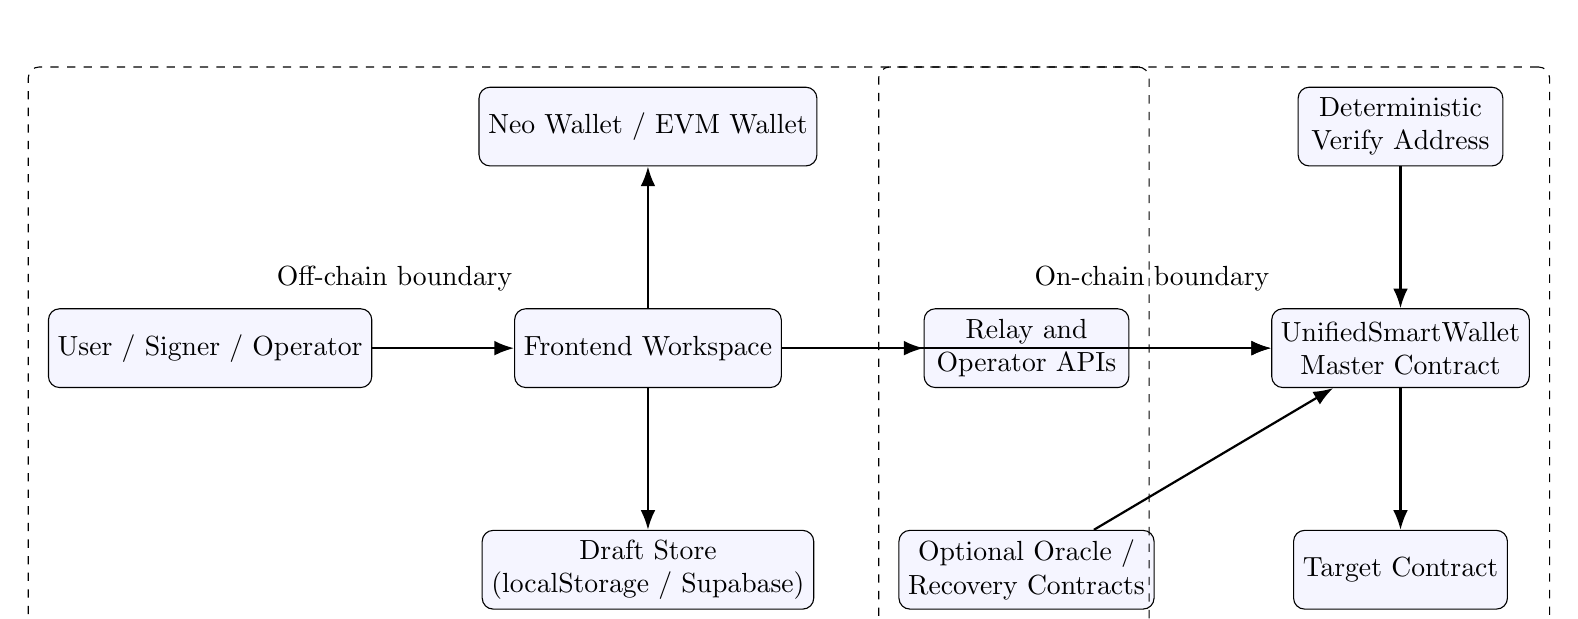
\begin{tikzpicture}[
  node distance=1.8cm and 1.8cm,
  box/.style={draw, rounded corners, align=center, minimum width=2.6cm, minimum height=1cm, fill=blue!4},
  trust/.style={draw, dashed, rounded corners, inner sep=0.25cm},
  arrow/.style={-{Latex[length=2.5mm]}, thick}
]

\node[box] (user) {User / Signer / Operator};
\node[box, right=of user] (frontend) {Frontend Workspace};
\node[box, below=of frontend] (drafts) {Draft Store\\(localStorage / Supabase)};
\node[box, above=of frontend] (wallets) {Neo Wallet / EVM Wallet};
\node[box, right=of frontend] (relay) {Relay and\\Operator APIs};
\node[box, right=of relay] (master) {UnifiedSmartWallet\\Master Contract};
\node[box, above=of master] (proxy) {Deterministic\\Verify Address};
\node[box, below=of master] (target) {Target Contract};
\node[box, below=of relay] (oracle) {Optional Oracle /\\Recovery Contracts};

\draw[arrow] (user) -- (frontend);
\draw[arrow] (frontend) -- (wallets);
\draw[arrow] (frontend) -- (drafts);
\draw[arrow] (frontend) -- (relay);
\draw[arrow] (frontend) -- (master);
\draw[arrow] (proxy) -- (master);
\draw[arrow] (relay) -- (master);
\draw[arrow] (master) -- (target);
\draw[arrow] (oracle) -- (master);

\node[trust, fit=(user)(frontend)(wallets)(drafts)(relay)] {};
\node[trust, fit=(proxy)(master)(target)(oracle)] {};
\node[above left=0.1cm and -0.1cm of frontend] {Off-chain boundary};
\node[above left=0.1cm and -0.1cm of master] {On-chain boundary};
\end{tikzpicture}
\caption{System architecture and trust boundaries}
\label{fig:architecture}
\end{figure}

\subsection{Contract Module Map}
\begin{table}[h!]
  \centering
  \caption{Master contract file responsibilities}
  \begin{tabularx}{\textwidth}{>{\raggedright\arraybackslash}p{0.38\textwidth}X}
    \toprule
    File & Responsibility \\
    \midrule
    \code{AbstractAccount.cs} & top-level entrypoints and shared integration glue \\
    \code{AbstractAccount.AccountLifecycle.cs} & account creation and deterministic address binding \\
    \code{AbstractAccount.StorageAndContext.cs} & storage layout, execution locks, transient context \\
    \code{AbstractAccount.ExecutionAndPermissions.cs} & policy-gated execution and target invocation \\
    \code{AbstractAccount.MetaTx.cs} & EIP-712 authorization and signer validation \\
    \code{AbstractAccount.Admin.cs} & role and threshold governance \\
    \code{AbstractAccount.Oracle.cs} & oracle-gated dome flow \\
    \code{AbstractAccount.Upgrade.cs} & deployer-only update path \\
    \bottomrule
  \end{tabularx}
\end{table}

\section{Account Model and State}
\subsection{Deterministic Addressing}
For each logical account, the system derives a deterministic verify script from the master-contract hash and \code{accountId}. The resulting script hash is the user-facing Neo address. No per-user contract deployment is required. A conforming implementation \must{} preserve the property that the verify address routes authorization back into the master contract.

\subsection{On-Chain State Categories}
\begin{table}[h!]
  \centering
  \caption{Principal on-chain state categories}
  \begin{tabularx}{\textwidth}{>{\raggedright\arraybackslash}p{0.24\textwidth}>{\raggedright\arraybackslash}p{0.18\textwidth}X}
    \toprule
    Category & Example Prefix & Purpose \\
    \midrule
    Admin set & \code{0x01} & serialized admin addresses \\
    Admin threshold & \code{0x02} & required admin signatures \\
    Manager set & \code{0x03} & serialized manager addresses \\
    Manager threshold & \code{0x04} & required manager signatures \\
    Blacklist / whitelist & \code{0x09}, \code{0x0B} & target policy constraints \\
    Max transfer & \code{0x0C} & amount ceilings for token transfers/approvals \\
    Verifier contract & \code{0x12} & optional external verifier logic \\
    Dome / oracle state & multiple scoped prefixes & inactivity recovery and oracle gating \\
    \bottomrule
  \end{tabularx}
\end{table}

\subsection{Off-Chain Collaboration State}
The collaboration layer stores draft-oriented coordination data rather than authorization truth. A draft \must{} be treated as a coordination artifact, not as an authority source. Likewise, a `.matrix` domain \must{} be treated as a discovery layer rather than the underlying source of account authorization.

\begin{table}[h!]
  \centering
  \caption{Off-chain draft data}
  \begin{tabularx}{\textwidth}{>{\raggedright\arraybackslash}p{0.25\textwidth}X}
    \toprule
    Field group & Meaning \\
    \midrule
    \code{operation\_body} & human/composer intent and contract-call shape \\
    \code{transaction\_body} & staged wrapped transaction details \\
    \code{signatures} & append-only collected signatures and approvals \\
    \code{metadata.activity} & bounded activity timeline (latest 100 entries) \\
    \code{metadata.submissionReceipts} & bounded receipt history (latest 12 entries) \\
    \code{share\_slug}, \code{collaboration\_slug}, \code{operator\_slug} & scoped URLs for read, sign, and operate roles \\
    \bottomrule
  \end{tabularx}
\end{table}

\section{Authorization and Execution Model}
\subsection{Verification Phase}
A valid deterministic proxy witness is not enough by itself. After hardening, the verify phase \must{} confirm that the top-level transaction script returns into the \AAsystem{} contract through an approved wrapper entrypoint.

\begin{figure}[h!]
\centering
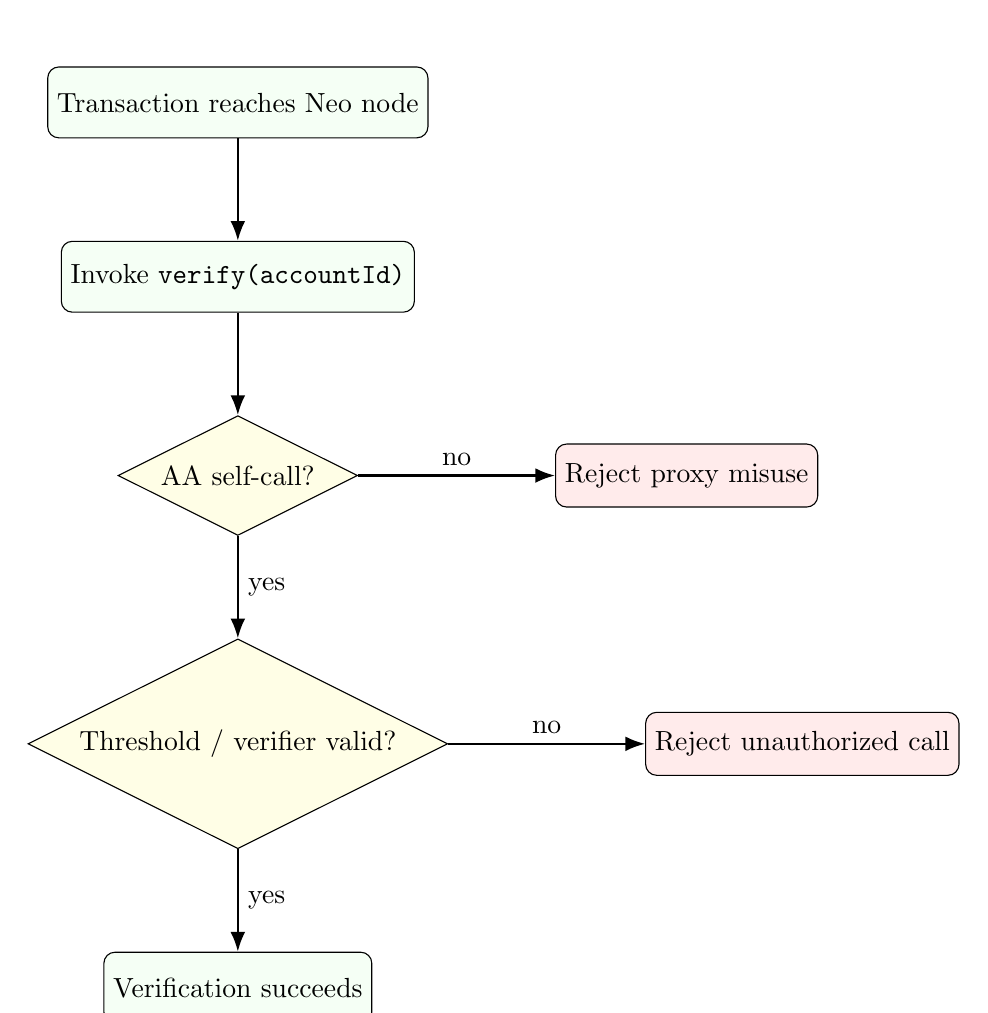
\begin{tikzpicture}[
  node distance=1.3cm and 1.0cm,
  verifybox/.style={draw, rounded corners, align=center, minimum width=2.8cm, minimum height=0.9cm, fill=green!4},
  decision/.style={draw, diamond, aspect=2, align=center, fill=yellow!10, inner sep=0.1cm},
  bad/.style={draw, rounded corners, align=center, minimum width=2.4cm, minimum height=0.8cm, fill=red!8},
  arrow/.style={-{Latex[length=2.5mm]}, thick}
]
\node[verifybox] (tx) {Transaction reaches Neo node};
\node[verifybox, below=of tx] (verify) {Invoke \code{verify(accountId)}};
\node[decision, below=of verify] (selfcall) {AA self-call?};
\node[bad, right=2.5cm of selfcall] (reject1) {Reject proxy misuse};
\node[decision, below=of selfcall] (auth) {Threshold / verifier valid?};
\node[bad, right=2.5cm of auth] (reject2) {Reject unauthorized call};
\node[verifybox, below=of auth] (pass) {Verification succeeds};
\draw[arrow] (tx) -- (verify);
\draw[arrow] (verify) -- (selfcall);
\draw[arrow] (selfcall) -- node[above] {no} (reject1);
\draw[arrow] (selfcall) -- node[right] {yes} (auth);
\draw[arrow] (auth) -- node[above] {no} (reject2);
\draw[arrow] (auth) -- node[right] {yes} (pass);
\end{tikzpicture}
\caption{Verification-phase decision flow}
\label{fig:verification}
\end{figure}

\subsection{Application Phase}
Once verification succeeds, the master contract enforces the application policy before calling the target contract. This separation between verification and application is fundamental to the design. Domain registration, when used during creation, is performed as a separate invocation in the same transaction batch rather than by expanding the master contract trust surface.

\begin{figure}[h!]
\centering
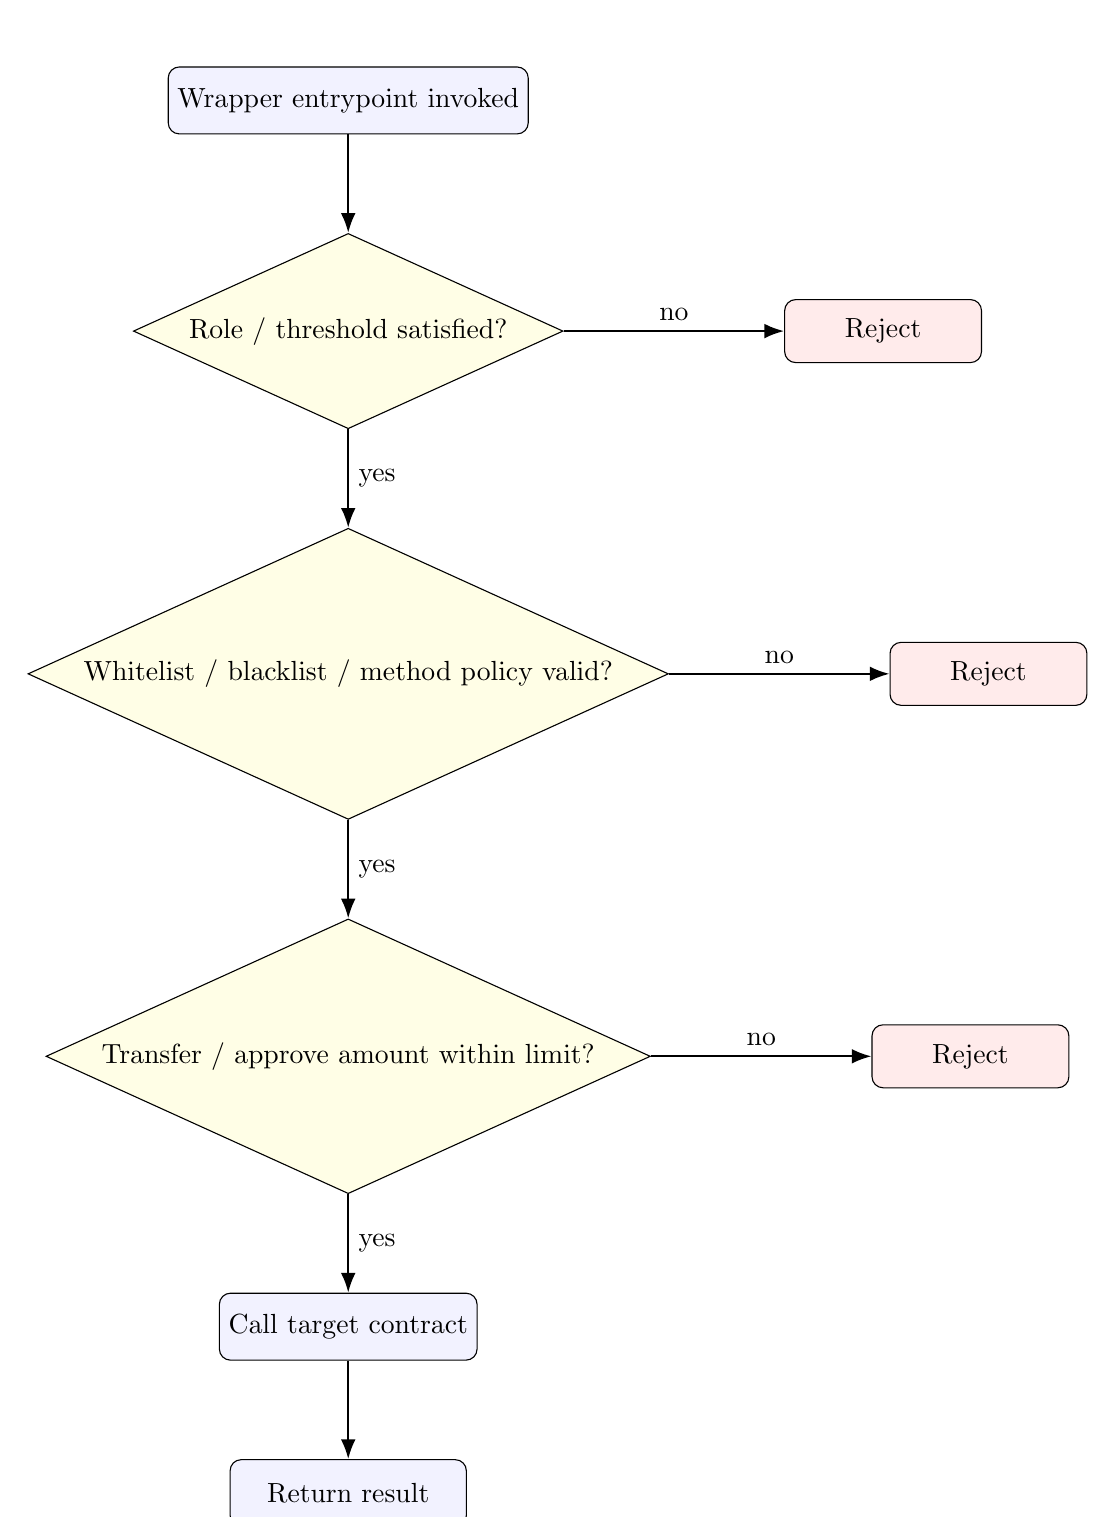
\begin{tikzpicture}[
  node distance=1.25cm and 0.8cm,
  procbox/.style={draw, rounded corners, align=center, minimum width=3.0cm, minimum height=0.85cm, fill=blue!5},
  decision/.style={draw, diamond, aspect=2.2, align=center, fill=yellow!10, inner sep=0.1cm},
  bad/.style={draw, rounded corners, align=center, minimum width=2.5cm, minimum height=0.8cm, fill=red!8},
  arrow/.style={-{Latex[length=2.5mm]}, thick}
]
\node[procbox] (entry) {Wrapper entrypoint invoked};
\node[decision, below=of entry] (role) {Role / threshold satisfied?};
\node[bad, right=2.8cm of role] (bad1) {Reject};
\node[decision, below=of role] (policy) {Whitelist / blacklist / method policy valid?};
\node[bad, right=2.8cm of policy] (bad2) {Reject};
\node[decision, below=of policy] (limit) {Transfer / approve amount within limit?};
\node[bad, right=2.8cm of limit] (bad3) {Reject};
\node[procbox, below=of limit] (call) {Call target contract};
\node[procbox, below=of call] (return) {Return result};
\draw[arrow] (entry) -- (role);
\draw[arrow] (role) -- node[above] {no} (bad1);
\draw[arrow] (role) -- node[right] {yes} (policy);
\draw[arrow] (policy) -- node[above] {no} (bad2);
\draw[arrow] (policy) -- node[right] {yes} (limit);
\draw[arrow] (limit) -- node[above] {no} (bad3);
\draw[arrow] (limit) -- node[right] {yes} (call);
\draw[arrow] (call) -- (return);
\end{tikzpicture}
\caption{Application-phase policy enforcement}
\label{fig:application}
\end{figure}

\section{Protocol Workflows}
\subsection{Workflow Classes}
The repository supports three major workflow classes:
\begin{enumerate}
  \item Native Neo wallet execution,
  \item EVM meta-transaction execution,
  \item collaborative draft creation, review, and submission.
\end{enumerate}

\subsection{End-to-End User Workflow}
\begin{figure}[h!]
\centering
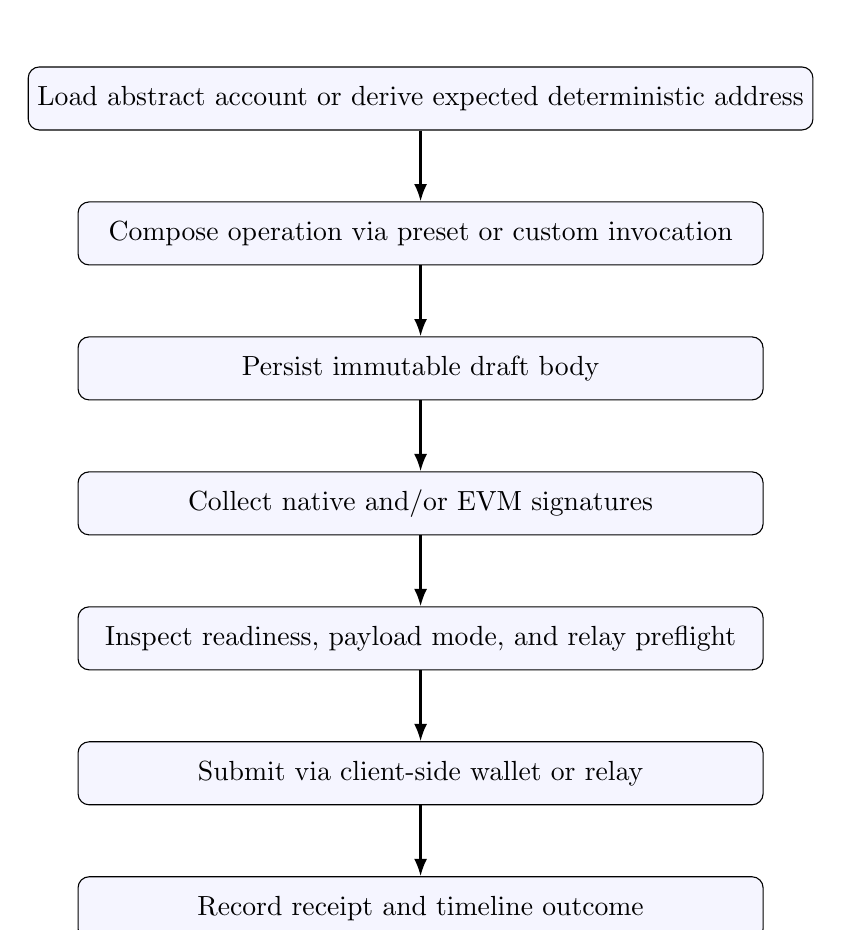
\begin{tikzpicture}[
  node distance=0.9cm,
  flowbox/.style={draw, rounded corners, align=center, minimum width=8.7cm, minimum height=0.8cm, fill=blue!4},
  arrow/.style={-{Latex[length=2.2mm]}, thick}
]
\node[flowbox] (a) {Load abstract account or derive expected deterministic address};
\node[flowbox, below=of a] (b) {Compose operation via preset or custom invocation};
\node[flowbox, below=of b] (c) {Persist immutable draft body};
\node[flowbox, below=of c] (d) {Collect native and/or EVM signatures};
\node[flowbox, below=of d] (e) {Inspect readiness, payload mode, and relay preflight};
\node[flowbox, below=of e] (f) {Submit via client-side wallet or relay};
\node[flowbox, below=of f] (g) {Record receipt and timeline outcome};
\draw[arrow] (a) -- (b);
\draw[arrow] (b) -- (c);
\draw[arrow] (c) -- (d);
\draw[arrow] (d) -- (e);
\draw[arrow] (e) -- (f);
\draw[arrow] (f) -- (g);
\end{tikzpicture}
\caption{Nominal user workflow}
\label{fig:workflow}
\end{figure}

\subsection{Execution Path Matrix}
\begin{table}[h!]
  \centering
  \caption{Execution path comparison}
  \begin{tabularx}{\textwidth}{>{\raggedright\arraybackslash}p{0.22\textwidth}>{\raggedright\arraybackslash}p{0.18\textwidth}>{\raggedright\arraybackslash}p{0.18\textwidth}X}
    \toprule
    Path & Signer Origin & Submission Origin & Notes \\
    \midrule
    Client-side native & Neo wallet & Browser wallet & simplest and default-safe path \\
    Relay preflight & Any prepared payload & Relay API & simulation only, no final broadcast \\
    Relay raw submission & pre-signed raw tx & Relay API & only when raw forwarding is explicitly enabled \\
    Meta invocation relay & EVM typed-data signatures & Relay signer & preserves EIP-712 UX while enforcing \AAsystem{} policy \\
    \bottomrule
  \end{tabularx}
\end{table}

\subsection{Collaborative Draft Flow}
A collaborative draft implementation \must{} preserve the following scope semantics:
\begin{itemize}
  \item public share links are read-only,\n  \item `.matrix` domain lookups are a discovery convenience and do not override on-chain account authority,\n  \item collaborator links are signature-only,
  \item operator links govern relay, receipt, and rotation actions,
  \item operator-class actions may be mediated by a signed server-side mutation path.
\end{itemize}

\section{Data Flow and State Model}
\subsection{System Boundary View}
\begin{figure}[h!]
\centering
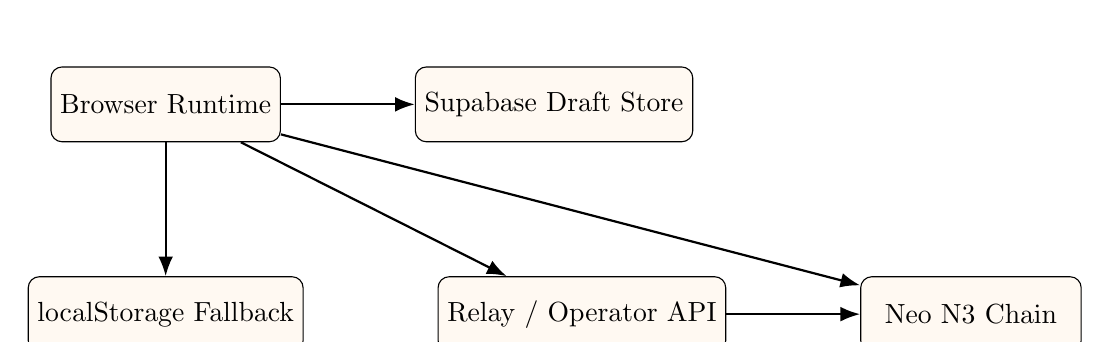
\begin{tikzpicture}[
  node distance=1.7cm and 1.7cm,
  box/.style={draw, rounded corners, align=center, minimum width=2.8cm, minimum height=0.95cm, fill=orange!5},
  arrow/.style={-{Latex[length=2.5mm]}, thick}
]
\node[box] (browser) {Browser Runtime};
\node[box, right=of browser] (supabase) {Supabase Draft Store};
\node[box, below=of browser] (local) {localStorage Fallback};
\node[box, right=of local] (relay) {Relay / Operator API};
\node[box, right=of relay] (chain) {Neo N3 Chain};

\draw[arrow] (browser) -- (supabase);
\draw[arrow] (browser) -- (local);
\draw[arrow] (browser) -- (relay);
\draw[arrow] (browser) -- (chain);
\draw[arrow] (relay) -- (chain);
\end{tikzpicture}
\caption{Data movement across off-chain and on-chain boundaries}
\label{fig:dataflow}
\end{figure}

\subsection{Authority Matrix}
\begin{table}[h!]
  \centering
  \caption{Data authority by boundary}
  \begin{tabularx}{\textwidth}{>{\raggedright\arraybackslash}p{0.22\textwidth}>{\raggedright\arraybackslash}p{0.28\textwidth}X}
    \toprule
    Boundary & Primary data & Authority characteristics \\
    \midrule
    On-chain master & roles, thresholds, nonce, policy, verifier state & authoritative, consensus-backed, final execution source \\
    Browser memory & active workspace and wallet session & ephemeral, user-local, not authoritative \\
    localStorage & local-only drafts and preferences & same-browser convenience only \\
    Supabase & draft body, append-only signatures, bounded activity and receipts & coordination state with scoped mutations \\
    Relay API & simulation, submission, signed operator mutations & helper boundary; must not redefine on-chain authority \\
    \bottomrule
  \end{tabularx}
\end{table}

\subsection{Retention and Mutability}
A conforming collaboration implementation \should{} preserve bounded metadata behavior:
\begin{itemize}
  \item latest 100 activity entries retained,
  \item latest 12 submission receipts retained,
  \item immutable draft body preserved independently from append-only signature history.
\end{itemize}

\section{Recovery Verifiers}
The repository includes dedicated recovery verifiers for social-recovery-style authorization patterns. These verifiers are separate from the main master contract and are intended to validate specialized recovery logic.

\begin{table}[h!]
  \centering
  \caption{Validated recovery verifier deployments on Neo N3 testnet}
  \begin{tabularx}{\textwidth}{>{\raggedright\arraybackslash}p{0.26\textwidth}>{\raggedright\arraybackslash}p{0.31\textwidth}X}
    \toprule
    Contract & Deployed hash & Model \\
    \midrule
    ArgentRecoveryVerifier & \code{0x260b204b109506140f6e20ef99d02c142d070f72} & guardian set with thresholded recovery flow \\
    SafeRecoveryVerifier & \code{0x06a7c50c2dd81f988e2e31b7fd721501008fbfa8} & modular threshold-based recovery with timelock parameterization \\
    LoopringRecoveryVerifier & \code{0x3ed17f73f19a89bc36e2dd82a19fc920aa2e54c7} & guardian-hash-based recovery with optional timelock behavior \\
    \bottomrule
  \end{tabularx}
\end{table}

The recovery verifier workflow in this repository additionally \must{} satisfy the following implementation constraints:
\begin{itemize}
  \item only validated \code{*.Fixed.cs} recovery sources are used for reproducible compilation,
  \item no plaintext WIF values are stored in repository documentation or helper scripts,
  \item official package-script validators exist for Argent, Safe, and Loopring,
  \item deployed hashes and txids are recorded in the repository validation record.
\end{itemize}

\section{Security Considerations}
\subsection{Core Invariants}
A conforming implementation \must{} preserve the following invariants:
\begin{enumerate}
  \item the deterministic verify address never replaces the master contract as the authority source;
  \item unsupported raw proxy-signed external spends are rejected;
  \item verification and application checks are both required for a valid execution;
  \item off-chain draft storage never bypasses on-chain authorization;
  \item operator-only actions remain narrower than general collaboration reads or signer mutations.
\end{enumerate}

\subsection{Hardening Measures Present in the Repository}
\begin{itemize}
  \item uncompressed meta-transaction public key length validation,
  \item relay and operator API rate limiting with \code{Retry-After} signaling,
  \item sanitized relay error responses,
  \item browser security headers in frontend deployment configuration,
  \item project/build isolation to prevent artifact contamination across contract trees.
\end{itemize}

\subsection{Operational Recommendations}
Operators \should{}:
\begin{itemize}
  \item verify runtime configuration before enabling relay submission,
  \item keep secrets server-side only,
  \item treat collaboration links as scoped capabilities and rotate them when exposed,
  \item record deploy txids, contract hashes, and validator outputs for all recovery contracts.
\end{itemize}

\section{Implementation and Deployment Notes}
\subsection{Runtime Configuration}
The repository distinguishes between browser-safe runtime hints and server-only secrets. Browser-exposed values inform UI features and endpoints, while signing keys and service-role credentials remain server-side.

\subsection{Repository Verification}
The repository verification script builds the main contract, regenerates contract artifacts, runs the contract tests, runs the frontend tests and build, performs a frontend production audit, and runs the SDK test suite. The main contract artifact generation now occurs through an isolated helper to avoid interaction with recovery build intermediates.

\subsection{Reference Workflow for Recovery Verifier Validation}
\begin{enumerate}
  \item rebuild recovery artifacts through the isolated helper,
  \item run local readiness checks,
  \item deploy with \code{neo-go contract deploy --await},
  \item record the hash and txid,
  \item run \code{npm run testnet:validate:recovery:all} with environment variables for all three deployed contracts.
\end{enumerate}

\section{Testnet Validation Summary}
The current repository state includes live Neo N3 testnet evidence for:
\begin{itemize}
  \item master-contract validation and hardened wrapper execution,
  \item recovery verifier deployment and basic on-chain validation,
  \item Safe and Loopring recovery validator package-script execution,
  \item full repository verification on the current branch tip.
\end{itemize}

\section{Conclusion}
The \aasystem{} combines deterministic addressing, shared-contract execution, scoped off-chain collaboration, relay-assisted submission, and specialized recovery verifiers into a cohesive policy-gated account abstraction model for Neo N3. The design prioritizes explicit trust boundaries, low per-account deployment overhead, and reproducible verification. The repository's current implementation and validation evidence support use by implementers and auditors as an operationally grounded reference system rather than a purely theoretical abstraction design.

\appendix
\section{Appendix A: Repository Documentation Map}
The following files complement this formal specification:
\begin{itemize}
  \item \code{README.md}
  \item \code{docs/INDEX.md}
  \item \code{docs/HOW\_IT\_WORKS.md}
  \item \code{docs/WORKFLOWS.md}
  \item \code{docs/DATA\_FLOW.md}
  \item \code{contracts/recovery/TESTNET\_VALIDATION\_2026-03-09.md}
\end{itemize}

\section{Appendix B: Recommended Reader Profiles}
\begin{itemize}
  \item \textbf{Operator}: focus on Sections 6, 7, 8, and 9.
  \item \textbf{Auditor}: focus on Sections 5, 6, 8, and the recovery verifier appendix.
  \item \textbf{Integrator}: focus on Sections 4, 6, 7, and 9.
  \item \textbf{Protocol engineer}: read the document in order.
\end{itemize}

\end{document}
